%%%%%%%%%%%%%%%%%%%%%%%%%%%%%%%%%%
%  Continuity and Discontinuity  %
%%%%%%%%%%%%%%%%%%%%%%%%%%%%%%%%%%

\section{Continuity and Discontinuity}

%%%%%%%%%%%%%%%%%%%%%%%%%%%%%%%%%%%%%%%%%%%%%%%%%%
%  Discussion: Examples of Dirichlet and Thomae  %
%%%%%%%%%%%%%%%%%%%%%%%%%%%%%%%%%%%%%%%%%%%%%%%%%%

\subsubsection*{Discussion (A deeper dive): Examples of Dirichlet and Thomae\footnote{Stephen Abbott - Understanding Analysis 4.1}}
Given a function $f$ with domain $A \subseteq \mathbb{R}$, we want to define continuity at a point $c \in A$ to mean that if $x \in A$ is chosen \textit{near c}, then $f(x)$ will be near $f(c)$. \\
Symbolically, we will say $f$ is continuous at $c$ if
$$ \lim_{x \to c} f(x) = f(c) $$
However, the problem is that, at present, it's not entirely clear what is meant by $ \lim_{x \to c} f(x) $. Let's define a function (Idea of German mathematitian Peter Lejuene Dirichlet) $g$ like this:\\
\begin{minipage}{0.45\textwidth}
    \begin{equation*}
        g(x)
        \begin{cases}
            1 & \text{if } x \in \mathbb{Q} \\
            0 & \text{if } x \notin \mathbb{Q}
        \end{cases}
    \end{equation*}
\end{minipage}
\begin{minipage}{0.45\textwidth}
    \centering
    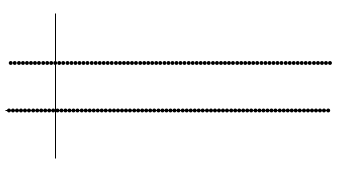
\includegraphics[scale=0.4]{Dirichlet g_x.png}
    \captionof{figure}{\small Dirichlet's Function, $g(x)$}
\end{minipage} \\~\\
Does it make sense to attach a value to the expression $\lim_{x \to 1/2} \ g(x)$? One idea is to consider a sequence $(x_n) \to 1/2$. Using our notion of limit of a sequence if we try to define $g(x_n)$  as simply the limit of the sequence $g(x_n)$, the limit depends on how the sequence $(x_n)$ is chosen. If each $x_n$ is rational, then \[
    \lim_{n \to \infty} g(x_n) = 1
\]
And if $x_n$ is irrational for each n, then \[
    \lim_{n \to \infty} g(x_n) = 0
\]
Generally speaking, we want the value of $\lim_{x \to c} g(x)$ to be independent of how we approach c. In this particular case, the definition of a functional limit that we agree on should lead to the conclusion that \[
    \lim_{x \to 1/2} g(x) \quad\text{does not exist}
\]
We can also realize that Dirichlet's function is not continuous at c = 1/2. In fact, the real significance of the function is that there's nothing unique about the point c=1/2. Because both $\mathbb{Q}$ and $\mathbb{Q}'$ are dense in the real line, it follows that for any $z \in \mathbb{R}$ we can find sequences $(x_n) \subseteq \mathbb{Q}$ and $(y_n) \subseteq \mathbb{Q}'$ such that \[
    \lim x_n = \lim y_n = z
\]
Because \[
    \lim g(x_n) \neq \lim g(y_n)
\]
the same line of reasoning reveals that $g(x)$ is not continuous at $z$. In fact, Dirichlet's function is a \textit{nowhere-continuous} on $\mathbb{R}$.
How about if we redefine the Dirichlet's function in the following way? \\
\begin{minipage}{0.45\textwidth}
    \begin{equation*}
        h(x) = 
        \begin{cases}
            x & \text{ if } x \in \mathbb{Q} \\
            0 & \text{ if } x \notin \mathbb{Q}
        \end{cases}
    \end{equation*}
\end{minipage}
\begin{minipage}{0.45\textwidth}
    \centering
    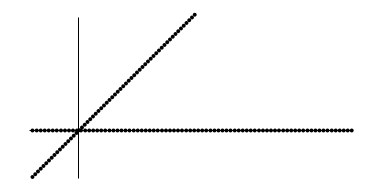
\includegraphics[scale=0.4]{Dirichlet h_x.png}
    \captionof{figure}{\small Modified Dirichlet's Function, $h(x)$}
\end{minipage} \\~\\
$h$ is not continuous at every point $c \neq 0$ in the same way. \\
But, when $c=0$, these two limits are both equal to $h(0)=0$. Regardless of how we construct a sequence $(z_n)$ converging to zero, the limit is always $\lim h(z_n)=0$. \\
This observation goes to the heart of what we want functional limits to entail. To assert that \[
    \lim_{x \to c} h(x) = L
\]
should imply that \[
    h(z_n) \to L \text{ for all sequences } (z_n) \to c
\]

\quad To this point, we've been discussing continuity of a function at a particular point in its domain. This is a significant departure from thinking of continuous founctions as curves that can be drawn without lifting the pen from the paper, and it leads to some fascinating questions. In 1875, K. J. Thomae discovered the function
\begin{equation*}
    t(x) = 
    \begin{cases}
        1 & \text{ if } x = 0 \\
        1/n & \text{ if } x = m/n \in \mathbb{Q}\backslash \{0\} \text{ is in lowest terms with n $>$ 0 } \\
        0 & \text{ if } x \notin \mathbb{Q}
    \end{cases}
\end{equation*}
\begin{figure}[ht]
    \centering
    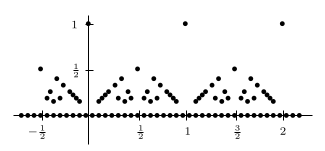
\includegraphics[scale=0.5]{Thomae.png}
    \captionof{figure}{\small Thomae's Function, $t(x)$}
\end{figure} \\
If $c \in \mathbb{Q}$, then $t(c) > 0$. Because $\mathbb{Q}'$ is dense in $\mathbb{R}$, we can find a sequence $(y_n)$ in $\mathbb{Q}'$ converging to c. The result is that \[
    \lim t(y_n) = 0 \neq t(c)
\]
and Thomae's function fails to be continuous at any rational point.\\
Let's try this argument on some irrational point like $c=\sqrt{2}$. All irrational values get mapped to $0$ by function $t$, so let's consider a sequence $(x_n)$ of rational numbers instead that converges to $\sqrt{2}$. So, the sequence of rational approximations for $\sqrt{2}$ might be \[
    \left( 1, \frac{14}{10}, \frac{141}{100}, \frac{1414}{1000}, \frac{14142}{10000}, \frac{141421}{100000}, ... \right)
\]
In this case, the sequence $t(x_n)$ begins, \[
    \left( 1, \frac{1}{5}, \frac{1}{100}, \frac{1}{500}, \frac{1}{5000}, \frac{1}{100000}, ... \right)
\]
The denominator of these fractions are getting larger and fast approaching $0 = t(\sqrt{2})$. This always happens. The closer a rational number is chosen to a fixed irrational number, the larger its denominator must necessarily be. Consequently, Thomae's function has the bizarre property of being continuous at every irrational point and discontinuous at every rational point on $\mathbb{R}$. \\

\quad Can there be examples of functions with the opposite property? If we're given some set $A \subseteq \mathbb{R}$, is it always possible to find a function that is continuous only on the set $A^c$? In each of our examples, the functions were defined to have erratic oscillations around points in the domain. What about we restrict our attention to somewhat less volatile functions like a \textit{monotinic} (A function which is either always increasing or always decreasing on a given domain) function? What might we be able to say about the set of discontinuities of a monotonic function on $\mathbb{R}$? \\~\\


%%%%%%%%%%%%%%%%
%  Continuity  %
%%%%%%%%%%%%%%%%

\subsection{Continuity}
\begin{definition}{Continuity}
    
    \\ A function $f(x)$ is said to be continuous at $x=a$ if,
    \begin{enumerate}[(i)]
        \item $\lim_{x \to a^-} f(x)$ exists
        \item $\lim_{x \to a^+} f(x)$ exists
        \item $f(x)$ is finite
        \item $\lim_{x \to a^-} f(x) = f(a) = \lim_{x \to a^+} f(x)$
    \end{enumerate}
\end{definition}

\begin{definition}{Cauchy's Definition of Continuity}
    
    A function $f:A \to \mathbb{R}$ is continuous at a point $c\in A$ if \[
        \forall \epsilon>0, \exists\delta>0 : \forall x\in A, |x-c|<\delta \implies |f(x)-f(c)|<\epsilon
    \]
\end{definition}

\begin{theorem}{Properties of Continuous Functions}
    
    Let $f(x)$ and $g(x)$ be two functions of $x$ each being continuous at $x=a$. For $\lim_{x \to a} f(x) = l$ and $\lim_{x \to a} g(x) = m$, the following statements are true:
    \begin{enumerate}[(i)]
        \item $ \lim_{x \to a} \{ f(x)\pm g(x) \} = \lim_{x \to a} f(x) \pm \lim_{x \to a} g(x) = f(a)\pm g(a) $
        \item $ \lim_{x \to a} \{ f(x)g(x) \} = \lim_{x \to a} f(x)\lim_{x \to a} g(x) = f(a)g(a) $
        \item $ \lim_{x \to a} \frac{f(x)}{g(x)} = \frac{\lim_{x \to a} f(x)}{\lim_{x \to a} g(x)} = \frac{f(a)}{g(a)} $
        \item If $f(x)$ is continuous in a closed interval, it's bounded in that interval
        \item A function wich is continuous in a closed interval attains at least once its least upper and greatest lower bounds.
        \item A continuous function wich has opposite sign at two points meets its domain vanishes at least once between these points.
        \item A continuous function $f(x)$ in the interval $(a,b)$ assumes at least once every value between $f(a)$ and $f(b)$, it being supposed that $f(a) \neq f(b)$.
        \item The converse of this theorem is not true i.e a function $f(x)$ which takes all values between $f(a)$ and $f(b)$ is not necessarily continuous in the interval $(a,b)$.
    \end{enumerate}
\end{theorem}

%%%%%%%%%%%%%%%%%%%
%  Discontinuity  %
%%%%%%%%%%%%%%%%%%%

\subsection{Discontinuity}

\begin{definition}{Discontinuous Function}
    
    A function $f(x)$ is said to be discontinuous for $x=a$ if $f(x)$ does not satisfy at least one of the conditions of continuity in Definition 2.1.1. \\~\\

    \underline{\textbf{Discontinuities are:}}
    \begin{enumerate}[(i)]
        \item Ordinary discontinuity / discontinuity of 1st kind
        \item Ordinary discontinuity / discontinuity of 2nd kind
        \item Removal discontinuity
        \item Mixed discontinuity
        \item Oscillatory discontinuity
        \item Infinite discontinuity
    \end{enumerate}
\end{definition}\vspace{5mm}

\underline{\textbf{A. Discontinuity of the first kind:}}
If the function $f(x)$ has finite limit, but  \[
    \lim_{h \to 0} f(a+h) \neq \lim_{h \to 09} f(a-h) \neq f(a)
\] the function is said to have ordinary discontinuity or discontinuity of the first kind at $x=a$. \\~\\

\underline{\textbf{B. Discontinuity of the second kind:}}
If both the limits of $f(x)$, i.e \[
    \lim_{h \to 0} f(a-h) \text{ and } \lim_{h \to 0} f(a+h)
\] do not exist for $x=a$ then $f(x)$ has a discontinuity of the second kind at $x=a$. \\~\\

\underline{\textbf{C. Mixed discontinuity:}}
If one of the limits of $f(x)$ exists, then the discontinuity of the function $f(x)$ at $x=a$ is called a mixed discontinuity. That is, if \[
    \lim_{h \to 0} f(a+h) = f(a) \text{ but } \lim_{h \to 0} f(a-h) \neq f(a)
\] then $f(x)$ is continuous on the right but it has an ordinary discontinuity on the left for $x=a$. In the same way, if \[
     \lim_{h \to 0} f(a-h) = f(a) \text{ but } \lim_{h \to 0} f(a+h) \neq  f(a)
\] then $f(x)$ is continuous on the right at $x=a$, and discontinuous on the left. \\~\\

\underline{\textbf{D. Removal discontinuity:}}
If \[
    \lim_{h \to 0} f(a+h) = \lim_{h \to 0} f(a-h) \neq f(a)
\] then the function $f(x)$ is said to have a removal discontinuity for $x=a$. \\~\\

\underline{\textbf{E. Infinite discontinuity:}}
If both the limits of $f(x)$ are infinite, the function $f(x)$ has an infinite discontinuity. That is, if \[
    \lim_{h \to 0^-} f(x) = \pm \infty \text{ or, } \lim_{h \to 0^+} f(x) = \pm \infty
\] then $f(x)$ is said to have an infinite discontinuity at $x=a$. \\~\\

\underline{\textbf{F. Oscillatory discontinuity:}}
A function $f(x)$ having a discontinuity at a point $x=a$ may oscillate finitely or infinitely to $\pm \infty$ as $x \to \infty$. In such a case, $f(x)$ has an Oscillatory discontinuity at $x=a$.

\begin{example}{Examine the continuity of the function $f(x)$ at $x=\frac{3}{2}$ where 
    \begin{equation*}
        f(x)
        \begin{cases}
            3-2x, &\text{ if } 0 \le x < \frac{3}{2} \\
            -3-2x, & \text{ if } x \ge \frac{3}{2}
        \end{cases}
    \end{equation*}
    }
    
    \[ \text{LHL } \lim_{x \to \frac{3}{2}^-} f(x) = \lim_{x \to \frac{3}{2}^-} \left\{ 3-2 \left( \frac{3}{2} \right) \right\} = 0 \]
    \[ \text{RHL } \lim_{x \to \frac{3}{2}^+} f(x) = \lim_{x \to \frac{3}{2}^+} \left\{ -3-2 \left( \frac{3}{2} \right) \right\} = -6 \]
    \[ f \left( \frac{3}{2} \right) = -3-2 \left( \frac{3}{2} \right)) = -6 \]
    \[ \therefore \text{RHL} = f\left(\frac{3}{2}\right) \neq \text{LHL} \]
    Thus $f(x)$ has a mixed discontinuity and it's discontinuous on the left.
\end{example}

\begin{example}{Show that the function \[
    f(x) = \frac{x-2}{x-1}
\] has an infinite discontinuity at $x=1$.}
    
    $f(x)$ has an infinite discontinuity at $x=a$, if &\lim_{x \to 0} \{ L_R - L_L \} = \infty$. Here,
    \[ f(1) = -\frac{1}{0} \text{ is undefined } \] Hence $f(x)$ is discontinuous at $x=1$. Now,
    \begin{align*}
        \lim_{h \to 0} \left| f(1+h) - f(1-h) \right| &= \lim_{h \to 0} \left| \frac{-1+h}{h} - \frac{-1-h}{-h} \right| \\
        &= \lim_{h \to 0} \left| -\frac{2}{/h} \right| \\
        &= \infty \\
    \end{align*}
    Hence, the discontinuity at $x=1$ is infinite.
\end{example}
